\subsection {Problema del agente viajero (TSP)}  
En TSP se tiene un número de nodos (ciudades, localidades, tiendas, empresas, etc.) que deben ser visitados por una entidad (persona, agente viajero, automóvil, avión, autobús, etc.), sin visitar 2 veces el mismo nodo. \\
\hspace*{1cm}Si se consideran 3 nodos (a, b y c) por visitar, entonces se tendrá una función de combinaciones sin repetición que se calcula con una función factorial ($n!$) es decir, se tendrán 6 posibles soluciones: abc, acb, bac, bca, cab, cba; para el caso de 4 nodos serian 24 combinaciones, para 10 nodos habría 3628800 combinaciones y así sucesivamente. En la figura \ref{fig:tsp1} se muestra otro ejemplo de los diferentes recorridos que puede dar un problema TSP, uno muestra un recorrido con un ineficiente resultado y otro con el resultado más eficiente.\\
    \begin{figure}[hbtp]
        \centering
            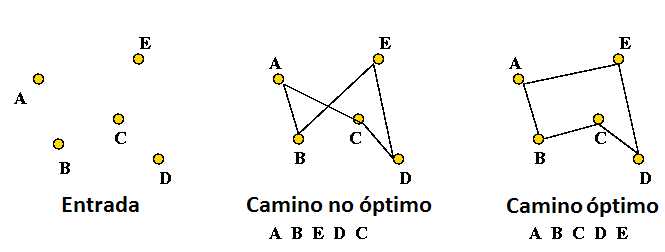
\includegraphics[width=1\textwidth]{MarcoTeorico/Imagenes/tsp1.png}
            \caption{Ejemplo de una instancia de TSP con 2 posibles soluciones.}                       
            \label{fig:tsp1}
    \end{figure} 
\hspace*{1cm}De acuerdo a \cite{[DANTZIG-RULKERSON]} la primera solución reportada para resolver una instancia del TSP fue en 1954, cuando Dantzig, Fulkerson y Johnson resolvieron una instancia de 49 ciudades.\\

\subsubsection{Características de TSP}
De acuerdo con \cite{[LENSTRA]}, TSP se encuentra clasificado como un problema de optimización combinatoria, es decir, en el problema en el que intervienen cierto número de variables donde cada variable puede tener N diferentes valores y cuyo número de combinaciones es de carácter factorial.\\
\hspace*{1cm}Para obtener una solución a una instancia del TSP se emplean diferentes métodos entre los cuales los principales se denominan heurísticas cuyo objetivo es generar soluciones de buena calidad en tiempos de cómputo mucho más pequeños (soluciones óptimas tiempo – respuesta). Las variables que han sido empleadas por la mayoría de los investigadores que dan solución a TSP son:

   \begin{itemize} 
      \item \textbf{Tiempo de recorrido entre ciudades:} Horas, minutos, días, semanas, etc.
      \item \textbf{Distancia de recorrido entre ciudades:} Metros, kilómetros, millas, milímetros, etc.
      \item \textbf{Costo de traslado:} Dinero, desgaste de las piezas, gasto de energía, etc.\\
   \end{itemize} 
   
\hspace*{1cm}Las variables que se pueden adoptar dependen de cada problema, por ejemplo:
   \begin{itemize} 
      \item \textbf{Circuitos electrónicos:} Cantidad de soldadura utilizada, menor espacio entre los puntos de soldadura de los circuitos, evitar el cruce entre las líneas de soldadura, tiempo de fabricación, distribución de los circuitos, entre otras.
      \item \textbf{Control de semáforos:} Número de semáforos (nodos), tiempo de traslado entre semáforos, cantidad de autos que pasan por un punto, entre otras variables.
      \item \textbf{Previsión del tránsito terrestre:} Puntos en una ciudad, cantidad de vehículos, tiempo de traslado, tipos de vehículos, horas pico, correlación entre variables, regresión lineal, etc.
      \item \textbf{Entrega de productos:} Peso de las entregas, número de entregas, nodos (domicilios) a visitar, recorridos, tiempos de traslado, tipo de vehículo, etc.
      \item \textbf{Estaciones de trabajo:} Secuencia de actividades, lugar de las herramientas (nodos), Tipo de herramientas, tiempo de uso, etc.
      \item \textbf{Edificación:} Puntos de edificación (construcciones), distancia entre las construcciones y los insumos, vehículos (grúas, camiones de volteo, etc.), cantidad de combustible que emplean, etc.
   \end{itemize} 

 
 \subsubsection {Algoritmo base}
 El TSP se puede modelar como un grafo cuyas aristas son los posibles caminos que puede seguir la entidad para visitar todos los nodos \cite{[ONCAN]}, y cuyo algoritmo se puede representar como en el pseudocódigo \ref{lst:codigo10}.\\
 
\begin{lstlisting}[language=HTML, caption=Algoritmo base del TSP., label=lst:codigo10]
* Definir el número de nodos, su posición y el costo por cada arista (i, j) donde i = ciudad 1 y j = ciudad 2.
* Elegir el nodo inicial i.
* Si el nodo más cercano no se ha visitado, visitar nodo j.
* Actualizar lista de nodos visitados.
* CostoTotal = CostoTotal + costo(i, j).
* Nodo i = nodo j.
* Repetir punto 3 hasta haber visitado todos los nodos.
\end{lstlisting}    
     
\subsubsection {Aplicaciones}
El TSP se puede emplear en cualquier situación que requiere seleccionar nodos en cierto orden que reduzca los costos:

\begin{itemize}
  \item \textbf{Reparto de productos:} Mejorar una ruta de entrega para seguir la más corta.
  \item \textbf{Transporte:} Mejorar el recorrido de caminos buscando la menor longitud.
  \item \textbf{Robótica:} Resolver problemas de fabricación para minimizar el número de desplazamientos al realizar una serie de perforaciones en un circuito impreso.
  \item \textbf{Turismo y agencias de viajes:} Aun cuando los agentes de viajes no tienen un conocimiento explícito del TSP, las compañías dedicadas a este giro utilizan un software que hace todo el trabajo. Estos paquetes son capaces de resolver instancias pequeñas del TSP.
  \item \textbf{Horarios de transportes laborales y/o escolares:} Estandarizar los horarios de los transportes es claramente una de sus aplicaciones, tanto que existen empresas que se especializan en ayudar a las escuelas a programarlos para optimizarlos en base a una solución del TSP.
  \item \textbf{Inspecciones a sitios remotos:} Ordenar los lugares que deberá visitar un inspector en el menor tiempo.
  \item \textbf{Secuencias:} Se refiere al orden en el cual n trabajos tienen que ser procesados de tal forma que se minimice el costo total de producción.
\end{itemize}
   
\subsubsection {Técnicas de solución}
El TSP puede resolverse de diferentes maneras:

\begin{itemize}
    \item \textbf{Enumeración de todas las soluciones factibles:} Es decir, listar todas las posibles soluciones al problema, calcular sus costos asociados e identificar, por comparación, cuál es la solución con el costo más conveniente.
 \item \textbf{Métodos exactos:} Intentan descartar familias enteras de posibles soluciones, tratando así de acelerar la búsqueda y llegar a una óptima. Los que más se usan para resolver el TSP son Ramificación y Acotamiento, y Ramificación y Corte.
 \item \textbf{Heurísticas:} Son métodos obtienen buenas soluciones en tiempos de cómputo muy cortos, aunque sin garantizar la solución única.
\end{itemize}

\hspace*{1cm}En la actualidad investigadores han propuesto diferentes estrategias para dar solución a TSP, de las cuales se pueden mencionar algunas técnicas empleadas:

\begin{itemize}
\item \textbf{Algoritmos genéticos:} La solución consiste en encontrar un individuo cuya combinación de genes (cada gen es una variable), den solución al problema de visitar todas las ciudades una vez. Otra solución es que cada gen es una ciudad y cuyo orden dependerá del orden en que serán visitadas.
\item \textbf{Redes neuronales:} Una red neuronal simula las conexiones entre los nodos (lugares por visitar), y cada recorrido por las diferentes neuronas genera al final un camino que involucra el tour por todas las ciudades visitadas una sola vez.
\item \textbf{Colonia de hormigas (ACO):} Las hormigas encuentran el camino más corto entre 2 puntos; para TSP, se considera el punto de inicio como el punto final, de esta manera, las hormigas deben recorrer todas las ciudades en un circuito, sin pasar 2 veces por la misma ciudad.
\item \textbf{Búsqueda Tabú:} Consiste en buscar el vecino próximo cuyos costos de traslado del nodo actual al siguiente sea el de menor costo en cuanto al uso de recursos.
\item \textbf{Combinación de propuestas:} Las técnicas de Inteligencia Artificial se pueden combinar para crear metaheurísticas conformando diferentes soluciones tales como: algoritmos genéticos con redes neuronales.
\end{itemize}

